% --- Template for thesis / report with tktltiki2 class ---
% 
% last updated 2013/02/15 for tkltiki2 v1.02

\documentclass[finnish]{tktltiki2}

% tktltiki2 automatically loads babel, so you can simply
% give the language parameter (e.g. finnish, swedish, english, british) as
% a parameter for the class: \documentclass[finnish]{tktltiki2}.
% The information on title and abstract is generated automatically depending on
% the language, see below if you need to change any of these manually.
% 
% Class options:
% - grading                 -- Print labels for grading information on the front page.
% - disablelastpagecounter  -- Disables the automatic generation of page number information
%                              in the abstract. See also \numberofpagesinformation{} command below.
%
% The class also respects the following options of article class:
%   10pt, 11pt, 12pt, final, draft, oneside, twoside,
%   openright, openany, onecolumn, twocolumn, leqno, fleqn
%
% The default font size is 11pt. The paper size used is A4, other sizes are not supported.
%
% rubber: module pdftex

% --- General packages ---

\usepackage[utf8]{inputenc}
\usepackage[T1]{fontenc}
\usepackage{lmodern}
\usepackage{microtype}
\usepackage{amsfonts,amsmath,amssymb,amsthm,booktabs,color,enumitem,graphicx}
\usepackage[pdftex,hidelinks]{hyperref}
\usepackage{algpseudocode}
\usepackage{float}

% Automatically set the PDF metadata fields
\makeatletter
\AtBeginDocument{\hypersetup{pdftitle = {\@title}, pdfauthor = {\@author}}}
\makeatother

% --- Language-related settings ---
%
% these should be modified according to your language

% babelbib for non-english bibliography using bibtex
\usepackage[fixlanguage]{babelbib}
\selectbiblanguage{finnish}

% add bibliography to the table of contents
\usepackage[nottoc]{tocbibind}
% tocbibind renames the bibliography, use the following to change it back
\settocbibname{Lähteet}

% --- Theorem environment definitions ---

\newtheorem{lau}{Lause}
\newtheorem{lem}[lau]{Lemma}
\newtheorem{kor}[lau]{Korollaari}

\theoremstyle{definition}
\newtheorem{maar}[lau]{Määritelmä}
\newtheorem{ong}{Ongelma}
\newtheorem{alg}[lau]{Algoritmi}
\newtheorem{esim}[lau]{Esimerkki}

\theoremstyle{remark}
\newtheorem*{huom}{Huomautus}


% --- tktltiki2 options ---
%
% The following commands define the information used to generate title and
% abstract pages. The following entries should be always specified:

\title{Vakaa avioliitto -ongelma}
\author{Anis Moubarik}
\date{\today}
\level{Tutkielma}
\abstract{Vakaa avioliitto -ongelma on tilanne jossa meillä on kaksi erillistä samansuuruista joukkoa joilla on jonkilainen mieltymys vastakkaisen joukon alkioista, kutsumme tilannetta avioliittopeliksi. Tutkielmassa tulee esille vakauden määritelmä ja sen vaikutuksia pareihin ja pariutuksiin ja kuinka näitä vakaita pariutuksia löydetään avioliittopeleistä. Näiden ohella esitellään Gale--Shapley-algoritmi, joka tuottaa yhden vakaan pariutuksen jokaiselle avioliittopelille.

Tutkielma käy läpi myös yleisimpiä muunnoksia alkuperäiseen ongelmaan, kuten erisuuruiset joukot ja parien kieltäminen. Sovelluksista tulee esille elinluovutus tapaukset, joka on muokattu vakaa huonetoveri -ongelma (\emph{stable roommate problem}), koulujen opiskelijavalinnat sekä opetussairaaloiden ja lääkettieteen opiskelijoiden pariutus.

Lopuksi käydään läpi strategioita sekä koalitioita avioliittopeleissä, kuinka ne vaikuttavat tai parantavatko ne strategioivien alkioiden pareja, kuinka koalitiot voivat manipuloida Gale--Shapley-algoritmiä ja onko petos kannattavaa koalitioissa.}

% The following can be used to specify keywords and classification of the paper:

\keywords{vakaat pariutukset, avioliittopeli, Gale--Shapley}
\classification{\textbf{Theory of computation} $\rightarrow$ \textbf{Algorithmic game theory}; \emph{Mathematics of computing} $\rightarrow$ \emph{Combinatoric problems;}} % classification according to ACM Computing Classification System (http://www.acm.org/about/class/)
                  % This is probably mostly relevant for computer scientists

% If the automatic page number counting is not working as desired in your case,
% uncomment the following to manually set the number of pages displayed in the abstract page:
%
% \numberofpagesinformation{16 sivua + 10 sivua liitteissä}
%
% If you are not a computer scientist, you will want to uncomment the following by hand and specify
% your department, faculty and subject by hand:
%
% \faculty{Matemaattis-luonnontieteellinen}
% \department{Tietojenkäsittelytieteen laitos}
% \subject{Tietojenkäsittelytiede}
%
% If you are not from the University of Helsinki, then you will most likely want to set these also:
%
% \university{Helsingin Yliopisto}
% \universitylong{HELSINGIN YLIOPISTO --- HELSINGFORS UNIVERSITET --- UNIVERSITY OF HELSINKI} % displayed on the top of the abstract page
% \city{Helsinki}
%


\begin{document}

% --- Front matter ---

\maketitle        % title page
\makeabstract
\tableofcontents  % table of contents
\newpage          % clear page after the table of contents


% --- Main matter ---

\section{Johdanto}
Vakaa avioliitto -ongelma (\emph{stable marriage problem}) sivuaa kombinatoriikkaa ja peliteoriaa. Ongelma on seuraava: Olkoon olemassa $n$ miestä ja $n$ naista ja miehet ovat pistäneet naiset järjestykseen mieluisimmasta parista huonoimpaan ja jokainen nainen on pistänyt miehet vastaavaan järjestykseen, tätä tilannetta kutsutaan \emph{avioliittopeliksi}. \emph{Pari} on tässä kontekstissa siis mies-nais pari, tätä kutsutaan myös \emph{avioliitoksi}. Tehtävänä on pariuttaa miehet ja naiset niin, että meillä ei ole kahta vastakkaisen sukupuolen henkilöä, jotka olisivat mielummin pari keskenään kuin pysyisivät avioliitossaan nykyisessä pariutuksessa. Avioliitot ovat vakaita, kun näitä \emph{estepareja} ei esiinny. Pariutus on joukko pareja ja parit voidaan pariuttaa Gale--Shapley-algoritmilla, joka esitellään myöhemmin. Vakaassa pariutuksessa on siis tarkoitus pariuttaa kahden joukon alkiot niin että jokin kriteeri täyttyy, alkuperäisessä vakaa avioliitto -ongelmassa tuo kriteeri on parien vakaus suhteessa alkioiden mieltymyksiin.

Ongelmalla on monia käytännön sovelluksia. Se voidaan yleistää kaikkiin \emph{kaksipuolisiin markkinoihin}, joissa eettisistä tai laillisista syistä ei käytetä vaihtovälineenä rahaa. Kaksipuolisilla markkinoilla tarkoitetaan tilannetta, jossa on olemassa alusta joka palvelee kahta erillistä ryhmää, jotka toimittavat toisilleen hyödykkeitä. Seuraavat markkinat ovat hyviä esimerkkejä: elinluovuttajat ja vastaanottajat, työntekijät ja työnantajat sekä opiskelijat ja korkeakoulut. Elinluovutusten tapauksessa haaste on se, että luovuttaja-potilas kaksikot eivät ole yhteensopivia, voimme kuitenkin käyttää vakaa avioliitto -ongelman ratkaisuja elinluovutuksissa. Jos on olemassa kaksikot $A$, $B$ ja $C$, eli jokainen kaksikoista sisältää luovuttajan ja potilaan, mutta syystä tai toisesta elin ei sovi potilaalle, voidaan soveltaa ratkaisuja tähän tapaukseen ja saada vakaita pariutuksia potilaitten ja luovuttajien välille. Oletetaan, että $A$:n luovuttaja sopii $B$:lle, $B$:n $C$:lle ja $C$:n $A$:lle, nyt saamme ketjun ja vakaan pariutuksen, jossa jokainen potilas saa uuden elimen. Näitä \emph{kaksipuolisia pariutusmarkkinoita} tutkimme paperissa.

Vastaan tulee myös pieniä variaatioita klassiseen avioliitto-ongelmaan, kuten erisuuruiset joukot ja alkioiden hyvin erilaiset mieltymykset, eli tapaukset joissa he eivät halua pariutua tietyn henkilön kanssa ollenkaan. Näissä tapauksissa vakauden määritelmää muokataan niin että pariutukset joissa alkio on ilman paria voi olla myös vakaa. Erisuuruisten joukkojen tapauksessa suuremman joukon alkioista jää pariuttamatta suuremman ja pienemmän joukon alkioiden lukumärään erotuksen verran alkioita.

Gale ja Shapley esittivät vuonna 1962 ilmestyneessä artikkelissa \cite{gale62a} algoritmin alkuperäiselle ongelmalle, joka löytää yhden vakaan pariutuksen jokaiselle olemassa olevalle avioliittopelille. Jokaisella avioliittopelillä on siis vähintään yksi vakaa pariutus. Algoritmi toimii oletuksena "miehet kosii, naiset hylkää" periaatteella. Tämä antaa kosijalle, tässä tapauksessa siis miehille, aina parhaan mahdollisen parin mitä he voivat pelin kontekstissa saada. Naisten kosiessa roolit tietysti vaihtuvat ja pariutukset ovat silloin naisille optimoituja.
Peliteoria tulee esille, kun joukkojen alkiot vääristelevät mieltymyksiään. Tähän vääristelyyn Gale--Shapley-algoritmi ei osaa puuttua ja se nostaakin kysymyksiä kuinka siihen pitäisi reagoida ja miten ylipäätään alkiot vääristelystä hyötyvät, jos hyötyvät ollenkaan.


\section{Vakaat pariutukset}
Olkooon $M$ \emph{miesten} joukko ja $N$ naisten joukko, missä $|M| = |N| = n$. Avioliitosta tai parista puhuttaessa tarkoitamme paria $(m, n) \in M \times N$. Avioliittopelissä jokaisella joukkojen alkiolla on mieltymykset toisen joukon alkioista parhaimmasta kumppanista huonoinpaan.

\begin{figure}[h!]
\caption{Yksi mahdollinen pari joukoista $M$ ja $N$}
\centering
	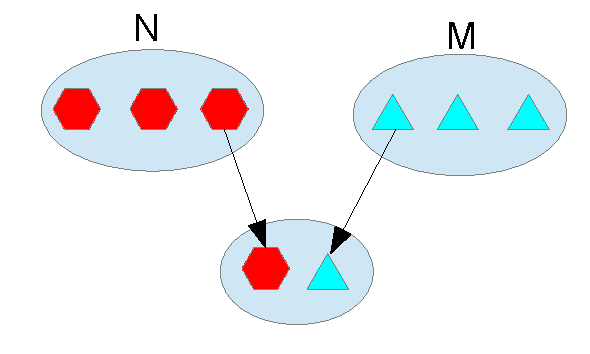
\includegraphics[scale=1.2]{paritutk}
\end{figure}

Olkoon meillä $m_1, m_2, m_3 \in M$ ja $n_1, n_2, n_3 \in N$. Mieltymykset voidaan kuvata esimerkiksi taulukossa. Järjestys on vasemmalta oikealle laskevassa järjestyksessä, eli miehelle $m_1$ miellyttävin pari olisi $n_2$.
\begin{table}[h!]
\begin{center}
	\begin{tabular}{ l | *{2}{c} r }
	 &  \\
	 \hline
 	 $m_{1}$ & $n_{2}$ & $n_{1}$ & $n_{3}$ \\
 	 $m_{2}$ & $n_{1}$ & $n_{2}$ & $n_{3}$ \\
 	 $m_{3}$ & $n_{3}$ & $n_{1}$ & $n_{2}$ \\
	\end{tabular}
	\caption{Miesten mieltymykset}
\end{center}
\end{table}

Mieltymyksiä voidaan myös kuvata transitiivisella relaatiolla $>$. Esimerkiksi miehen $m_1$ mieltymykset voidaan näyttää seuraavasti: $n_2 >_{m} n_1 >_{m} n_3$, relaatio on myös transitiivinen eli $n_2 >_{m} n_3$ pätee.

Pariutus $\mu$ on joukko $\mu \subseteq M \times N$,joka tulkittuna funktioksi on  $\mu : M \mapsto N$. Alkion $m$ paria pariutuksessa $\mu$ merkitään seuraavasti $p_{\mu}(m)$.

\begin{maar}
Pariutus $\mu$ on \emph{vakaa}, jos ei ole olemassa kaksikkoa $m_1$ja  $n_2$, jolle
\begin{enumerate}
	\item $n_2 >_{m_{1}} p_{\mu}(m_1)$, ja
	\item $m_1 >_{n_{2}} p_{\mu}(n_2)$
\end{enumerate}
\begin{figure}[h!]
\caption{Kuva epävakautta aiheuttavasta kaksikosta}
\centering
	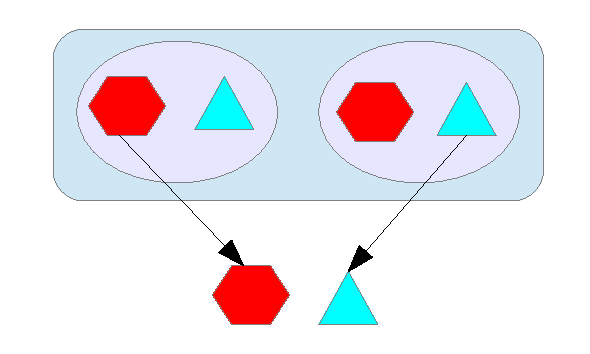
\includegraphics[scale=1.2]{vakaatutk}\label{epävakaa}
\end{figure}

Kuvassa \ref{epävakaa} meillä on pariutus, jossa on kaksi paria. Ensimmäisen parin nainen ja toisen parin mies pitävät toisistaan enemmän kuin omista pareistaan ja tämä aiheuttaa epävakautta.

\begin{ong}[Vakaa pariutus]
Löytää  vakaa pariutus joukoille $N$ ja $M$.
\end{ong}
\end{maar}

Pariutuksilla ja pareilla on erillaisia ominaisuuksia. Paras-miehelle pari on pari, jossa mies saa haluamansa naisen ja vastaavasti paras-naiselle pari on pari, jossa nainen saa haluamansa miehen. Pariutuksissa voi esiintyä jommankumman joukon ylivaltaa, jos kaikilla $j \in N$, $j$ saavat haluamansa parin, tätä kutsutaan $N$-joukon ylivallaksi ja samoin kaikilla $i \in M$, $i$ saavat haluamansa parin, tällöin se on $M$-joukon ylivalta. Joskus ylivaltoja kutsutaan myös \emph{nais}- tai \emph{miesylivallaksi}. Jos ylivaltaa ei synny pariutuksessa, voidaan pariutusta kutsua ylivaltavapaaksi.
Päinvastoin jos mies tai nainen saa huonoimman tai vähiten haluamansa parin, kutsutaan sitä \emph{huonoin-naiselle} tai -\emph{miehelle} pariksi. Samoin paria kutsutaan huonoin-naiselle tai -miehelle pariksi jos kaikki jommankumman joukon alkioista saavat vähiten haluamansa parit.

Esittelemme myöhemmin teoreeman, jonka mukaan jokaisesta avioliittopelistä löytyy ainakin yksi vakaa pariutus. Ensin kuitenkin esittelemme algoritmin joka tarkastaa pariutuksen vakauden.
Olkoon $m \in M$ ja $n \in N$ ja $\mu$ pariutus.
\begin{alg}
\begin{enumerate}
	\item Kaikilla $n$ siten että $m$ suosii naista $n$ enemmän kuin omaa paria $p_{\mu}(m)$
	\item Jos $n$ suosii miestä $m$ enemmän kuin omaa paria $p_{\mu}(n)$, ilmoitetaan että pariutus $\mu$ ei ole vakaa.
	\item Muuten ilmoitetaan että pariutus on vakaa.
\end{enumerate}
\end{alg}

Etsimme siis tapauksia jossa mies suosii naista enemmän kuin omaa pariaan pariutuksessa $p_\mu$.
Jos löydämme tälläisen miehen, tarkastelemme jos nainen jota hän suosii, suosii myös miestä enemmän kuin pariaan, jos tämä pitää paikkansa, ei pariutus voi olla vakaa.
Huonoimmassa tapauksessa käymme läpi kaikki miehet ja kaikki naiset paitsi yhden, eli $x\cdot(x-1)$, tästä saamme aikavaativuudeksi $O(x^2)$.

\section{Gale--Shapley-algoritmi}
Avioliittopelistä löytyy aina ainakin yksi vakaa pariutus. Gale--Shapley-algoritmi on yksinkertainen algoritmi, joka tuottaa vakaan parituksen avioliittopelille. Esittelemme algoritmin ja näytämme, että se päättyy aina.
\begin{alg} \cite[p. 13]{gale62a} \label{gsalg}.
\begin{enumerate}
	\item Miehet aloittavat kosimalla mieltymyksiltään parasta naista.
	\item Naiset hylkäävät kaikki paitsi parhaiten sijoitetun miehen.
	\item Nainen ei hyväksy miestä vaan jättää miehen \emph{langan} päähän siltä varalta että parempi mies kosisi häntä
	\item Hylätyt miehet kosivat mieltymyksiltään toisiksi parasta naista.
	\item Naiset hylkäävät kaikki paitsi parhaan vaihtoehdon
	\item Niin kauan kuin joku naisista ei ole saanut kosintaa, tulee hylkäyksiä ja uusia kosintoja. Lopuksi jokaista naista on kosittu, koska mies ei voi kuin kerran kosia samaa naista.
	\item Viimeinen nainen on saanut kosinnan ja kosimisvaihe on päättynyt. Jokainen nainen hyväksyy langan päässä olevan kosijan
\end{enumerate}
\end{alg}


\begin{lau}
Algoritmi \ref{gsalg} pysähtyy kaikilla söytteillä
\begin{proof}
Mies ei voi jäädä ilman paria. Nainen voi hylätä vain jos hänellä on langan päässä mies (ensimäisellä kierroksella naisen on siis valittava paras vaihtoehto langan päähän, hän ei voi hylätä kaikkia kosijoita), ja kun hänellä on langan päässä mies hänestä ei tule missään vaiheessa vapaata algoritmin suorittamisessa.
Jos viimeinen nainen jota kositaan hylkää miehen, tarkoittaisi tämä sitä, että jokaisella naisella olisi mies jo langan päässä. Mutta naisia ja miehiä on sama määrä ja yksikään mies ei voi olla kahden naisen langan päässä, niin jokainen miehistäkin pitäisi olla lankojen päässä, mikä on ristiriita.
Jokainen iteraatio sisältää yhden kosinnan eikä yksikään mies kosi samaa naista kahta kertaa, joten iteraatioiden määrä on $n^2$.
\end{proof}
\end{lau}
Algoritmi on siis päättyvä. Nyt siis päättyminen on selvää, mutta onko pariutukset aina vakaita?
Todistetaan tämä.
\begin{lau}
Ovatko Algoritmin \ref{gsalg} tuottamat pariutukset aina vakaita?
\begin{proof}\cite[p. 588]{gale62a}
Olkoon meillä mies $m$ ja nainen $n$ ja oletetaan, että he eivät ole pari pariutuksessa $\mu$. Oletetaan myös, että $n >_{m} p_{\mu}(m)$. Miehen $m$ on siis jossain vaiheessa algoritmiä kosia naista $n$ ja naisen $n$ on pitänyt jossain vaiheessa hylkää $m$ paremman miehen tieltä. On siis selvää, että $n$ suosii omaa pariaan pariutuksessa $\mu$ miehen $m$ sijaan, eikä epävakautta voi syntyä.
\end{proof}
\end{lau}
Algoritmi tuottaa tälläisenään miehelle optimaalisia tuloksia, eli tällä algoritmilla tuotettu pariutus on kyseiselle miehille paras mahdollinen mitä he siinä kyseisessä avioliittopelissä tulevat saamaan.
Naisille optimaalisia tuloksia voidaan saada, kun osat vaihdetaan päittäin algoritmissä.

\section{Vakaitten pariutusten joukko}
Gale-Shapley algoritmi tuottaa meille yhden vakaan pariutuksen, mutta niitä voi olla enemmän.
Olkoon meillä pariutus $\mu$ ja $\delta$. Henkilö $x$ suosii pariutusta $\mu$ pariutukseen $\delta$ nähden, jos $x$ suosii enemmän pariaan $\mu$ pariutuksessa kuin $\delta$ pariutuksessa. Henkilölle voi olla myös välinpitämätön pariutuksista, jos molemmat antavat hänelle yhtä hyvän parin.

\begin{lau} \cite[p. 18]{gusfield1989stable}\label{lause-guspref}
	Olkoon $\mu$ ja $\delta$ vakaita pariutuksia, ja oletetaan että $m$ ja $n$ ovat pari pariutuksessa $\mu$ muttei $\delta$:ssa. Nyt jompikumpi henkilöistä $m$ ja $n$ suosii pariutusta $\mu$ enemmän kuin pariutusta $\delta$ ja toinen pariutusta $\delta$ enemmän kuin pariutusta $\mu$.
\end{lau}
Sivuutamme todistuksen.
Tästä seuraa nyt, se että jos $\mu$ ja $\delta$ ovat vakaita pariutuksia samalle avioliittopelille, niin henkilöiden määrä jotka suosivat pariutusta $\mu$ on sama kuin henkilöiden määrä jotka suosivat pariutusta $\delta$.
Esitellään hieman myös notaatiota ylivalloille, tässä yhteydessä keskitymme miesylivaltaan.
Vakaa pariutus $\mu$ dominoi vakaata pariutusta $\delta$,jos jokainen mies saa vähintään yhtä hyvän parin pariutuksessa $\mu$ kuin $\delta$, merkitään sitä $\mu \preceq \delta$.
Jos meillä on miesylivalta se tarkoittaa sitä, että naisten kosiessa on oltava naisylivalta, joka merkitään seuraavasti $\mu \succeq \delta$. Olkoon $\mathcal{M}$ kaikkien pelin vakaiden pariutusten joukko avioliittopelissä. $(\mathcal{M}, \preceq)$ on osittain järjestetty joukko.  Merkitsemme sitä seuraavasti $(\mathcal{M}, \preceq)$.
Seuraava korollaari seuraa teoreemasta \ref{lause-guspref}

\begin{kor}
Miehen näkökulmasta pariutus $\mu$ hallitsee pariutusta $\delta$, joss pariutus $\delta$ hallitsee pariutusta $\mu$ naisten näkökulmasta. \emph{Nais-orientoitunut} ylivalta relaatio on käänteinen, merkinnällä $\succeq$, mies-orientoituneeseen nähden. Tämä on myös osittain järjestetty joukko ja se merkitään seuraavasti $(\mathcal{M}, \succeq)$. 
\end{kor}

\subsection{Vakaitten pariutusten määrä}
Haluamme nyt näyttää, että vakaita pariutuksia on eksponentiaalinen määrä. Joten jos käytämme brute-force algoritmia löytääksemme kaikki vakaat pariutukset, joudumme tyytymään eksponentiaaliseen aikavaativuuteen.

\begin{lem} \cite[p. 23]{gusfield1989stable} \label{lemma-koko}
Olkoon meillä vakaat avioliittopelit kooltaan $m$ ja $n$ ja vastaavasti olkoon $x$ ja $y$ vakaiden pariutuksien määrä avioliittopeleissä. On olemassa peli jonka koko on $m \cdot n$, jolla on vähintään $\max(xy^m, yx^n)$ vakaata pariutusta.
\end{lem}
Lemman todistus löytyy lähteestä, sivuutamme sen tässä.

\begin{lem}\cite[p. 24]{gusfield1989stable}
Jokaiselle $n \geq 0$, missä $n$ on kahden potenssi, on olemassa vakaa avioliittopeli jonka koko on $n$ ja sisältää vähintään $2^{n-1}$ vakaata pariutusta
\end{lem}
\begin{proof}
Todistus induktiolla. Kun pelin koko on 1, eli alkioiden lukumäärä on 1, niin $n = 2^0$ triviaali tapaus, eli vakaita pariutuksia on yksi. Oletetaan tulos todeksi tapauksessa $n = 2^k$, käytämme Lemmaa \ref{lemma-koko}, missä $i = 2$, avioliittopeli jonka koko on siis 2. Molemmat mahdolliset pariutukset ovat vakaita, joten $x = 2$ ja induktio-oletuksen mukaan $y = 2^{2^{k-1}}$. Joten Lemman \ref{lemma-koko} perusteella on olemassa peli jonka koko on $2 \cdot 2^k = 2^{k+1}$, jolla on vähintään $\max(2 \cdot (2^{2^{{k}}-1})^2, 2^{2^{k}-1} \cdot 2^{2^{k}}) = 2^{2^{k+1}-1})$ vakaata paritusta.
\end{proof}

\section{Laajennettu Gale--Shapley-algoritmi}
Tämä algoritmi sieventää alkioiden mieltymyslistoja poistamalla pareja, jotka eivät kuulu mihinkään vakaaseen pariutukseen. Poistamalla pari $(m, n)$ tarkoitetaan sillä sitä että $n$ poistetaan miehen $m$ mieltymyslistalta (\emph{preference list}) ja $m$ naisen $n$ listalta.

\begin{alg}\cite{gusfield1989stable}[p. 16]\label{alg2}
	\begin{enumerate}
		\item Alustetaan jokainen henkilö vapaaksi.
		\item Niin kauan kuin joku mies $m$ on vapaa,
		\item valitaan ensimmäinen nainen miehen listalta.
		\item Jos nainen $n$ on jo "kihloissa" miehen $p$ kanssa, vapautetaan $p$ ja pariutetaan $m$ kihloihin naisen $n$ kanssa.
		\item Poistetaan jokainen pari $(m^{'}, n)$, missä $m^{'}$ on $m$:n seuraaja $n$ mieltymyslistalla.
	\end{enumerate}
\end{alg}

Tässä algoritmissä, kun mies kosii naista kosinta hyväksytään aina. Koska jos nainen $n$ on jo kihloissa jonkun miellyttävämmän miehen kanssa, kuin $m$ olisi pari $(m, n)$ poistettu.
Algoritmi pysähtyy, kun jokainen on kihloissa. Huomaamme myös, että algoritmin lopettaessa jokainen mies on kihloissa listalla ensimmäisenä olevan naisen kanssa ja jokainen nainen taas kihloissa listalla viimeisenä olevan miehen kanssa.

Kutsumme algoritmin tuottamaa mieltymyslistaa, jossa miehet kosivat, \emph{mies-orientoituneeksi Gale--Shapley listaksi} tai \emph{MGS-listaksi}. Vastaavasti, jos miesten ja naisten roolit algoritmissä vaihdetaan kutsutaan tuotettua listaa \emph{NGS-listaksi}. Lopuksi jos otamme henkilön MGS- ja NGS-listasta leikkauksen saamme GS-listan.

\begin{lau}\cite{gusfield1989stable}[p. 16]
	Annettulle avioliittopelille pätee, että
	\begin{itemize}
		\item kaikki vakaat pariutukset ovat GS-listassa,
		\item Yksikään pari, joka ei ole GS-listalla ei voi estää pariutusta GS-listalta,
		\item mies-optimaalisissa (vastaavasti nais-optimaalisissa) pariutuksissa jokainen mies on pariutettu ensimmäisen (vastaavasti viimeisen) naisen kanssa hänen GS-listalta ja jokainen nainen viimeisen (vastaavasti ensimmäisen) miehen kanssa naisen listalta.
	\end{itemize}
\end{lau}


\section{Erisuuruiset joukot}
Aikaisemmat tulokset pätevät myös, kun meillä on kaksi joukkoa joiden alkioiden määrä on erisuuri. Oletamme, että henkilö haluaa olla ennemmin naimisissa kuin naimaton.
Olkoon $M$ miesten joukko ja $N$ naisten joukko, ja $|M| = n_x < n_y = |N|$. Pariutus $\mu$ on epävakaa, jos on olemassa mies $m \in X$ ja nainen $n \in Y$ siten että

\begin{enumerate}
	\item $m$ ja $w$ eivät ole pari pariutuksessa $\mu$,
	\item $m$ on joko ilman paria $\mu$:ssä tai suosii naista $w$ enemmän kuin pariaan pariutuksessa $\mu$, ja
	\item $w$ on joko ilman paria $\mu$:ssä tai suosii miestä $m$ enemmän kuin pariaan pariutuksessa $\mu$.
\end{enumerate}
Jokainen vakaa pariutus koostuu $n_x$:stä järjestettyjä pareja, missä $n_x - n_y$ on naimattomien naisten määrä.

\begin{lau}\cite[p. 26]{gusfield1989stable}.
Avioliittopelissä jossa meillä on erisuuruiset joukot, on olemassa vähintään yksi vakaa pariutus, jossa pienemmän joukon kaikki alkiot saavat parin. Jokainen pienemmän joukon alkio on vakaassa pariutuksessa ja suuremman joukon alkiot on jaettu kahteen osajoukkoon, toisen osajoukon alkiot ovat vakaassa pariutuksessa ja toisen osajoukon alkiot eivät ole pariutuksessa ollenkaan.
\end{lau}

Voimme muokata algoritmia \ref{gsalg}. Jos meillä on $x$ määrä miehiä ja $y$ määrä naisia, ja $x > y$, muokataan algoritmin 6. kohtaa ja päätetään, kun $x$ määrä naisia on kosittu. Jos taas $x < y$, niin algoritmi toimii normaalisti.


\section{Parien kieltäminen}
Jos henkilön on mahdollista ilmoittaa, että yksi tai useampi ei kelpaa hänelle vastakkaisen sukupuolen joukosta, on hänen mieltymyslistansa aito osajoukko vastakkaisen sukupuolen joukosta. Näinollen mies ja nainen voidaan pariuttaa ainoastaan jos he ovat hyväksyttäviä toisillensa.

Tässä tapauksessa vakaa pariutus voi olla osittainen tarkoittaen että kaikkien henkilöiden ei tarvitse olla pariutettu, jotta pariutus olisi vakaa. Osittainen pariutus $\mu$ on epävakaa, jos on olemassa mies $m$ ja nainen $n$ siten että
\begin{enumerate}
	\item $m$ ja $n$ eivät ole pari pariutuksessa $\mu$, mutta molemmat hyväksyisivät toisensa,
	\item $m$ on joko pariuttamaton tai suosii naista $n$ enemmän kuin hänen pariaan pariutuksessa $\mu$,
	\item $n$ on joko pariuttamaton tai suosii miestä $m$ enemmän kuin hänen pariaan pariutuksessa $\mu$.
\end{enumerate} 
Mieltymykset voidaan myös laajentaa koskemaan pariutuksia, eli henkilö suosii pariutusta jossa hänellä on pari verratuna pariutukseen jossa hän jää ilman paria.

\begin{lau}
Avioliittopelissä, joka sallii parien kieltämisen on miehet ja naiset jaettu kahteen joukkoon -- niihin joilla on pari kaikissa pariutuksissa ja niihin joilla ei ole yhtään paria missään pariutuksessa.
\end{lau}

\begin{proof}\cite[p. 27]{gusfield1989stable}
Olkoon kaksi eri vakaata pariutusta $\mu$ ja $\delta$, määrittelemme suunatun verkon $G = G(\mu, \delta)$, jossa solmu esittää yhtä henkilöä. Jokaiselle miehelle $m$ jolla on pari pariutuksessa $\mu$ on olemassa suunnattu kaari $m$:stä pariin $p_{\mu}(m)$. Ja jokaiselle naiselle $n$ jolla on pari pariutuksessa $\delta$ on olemassa suunnattu kaari $n$:stä pariin $p_{\delta}(n)$.
Jokaisella solmulla on verkossa $G$ enintään yksi tuleva ja lähtevä kaari.

Oletetaan nyt ristiriitaisesti, että $m$ on pariutettu naisen $n$ kanssa pariutuksessa $\mu$ muttei pariutuksessa $\delta$. On olemassa uniikki suunnaattu polku verkossa $G$ joka alkaa solmusta $m$ ja koska jokaisella solmulla on enintään yksi sisääntuleva kaari, ja $m$:llä on 0 sisääntulevaa kaarta, polku ei voi olla syklinen. Joten polun on päätyttävä mieheen joka on pariutettu $\delta$:ssa muttei $\mu$:ssa, eli $m$ suosii pariutusta $\delta$ ennemmin kuin pariutusta $\mu$, tai naiseen $n$ joka on pariutettu $\mu$:ssa muttei $\delta$:ssa $n$ suosii siis pariutusta $\mu$ ennemmin kuin pariutusta $\delta$.

Mutta koska $m$ suosii pariutusta $\mu$ pariutuksen $\delta$ sijaan, seuraa Lauseen \ref{lause-guspref} mukaan, että $n$ suosii pariutusta $\delta$ pariutuksen $\mu$ sijaan, ja Lausetta \ref{lause-guspref} soveltamalla polkuun huomaamme, että jokainen mies suosii pariutusta $\mu$ ja jokainen nainen pariutusta $\delta$. Joten kahdesta mahdollisesta reitistä, jossa polku voisi päättyä johtaa molemmat ristiriitaan.
\end{proof}

\section{Parien yhdentekeväisyys}
Voidaan hyväksyä myös tilanteita, joissa alkioiden mieltymyslistat eivät ole ehdottomasti sijoitettuja, eli alkio voi pitää yhdestä alkiosta yhtä paljon kuin toisesta. Toisin sanoen alkiolle on yhdentekevää kumman parin kanssa hänet pariutetaan. Avataan vakauden määritelmää. Jos meillä on nainen ja mies, jotka eivät ole pari, mutta pitävät toisistaan enemmän/yhtäpaljon kuin omista pareistaan kyseisessä pariutuksessa, on pariutus epävakaa. Kutsutaan pariutusta tämän kriteerin perusteella \emph{super-vakaaksi} (\emph{super-stable}) \cite{gusfield1989stable}. Tilanteessa jossa on olemassa täysi välinpitämättömyys emme voi löytää yhtään super-vakaata pariutusta.

Toinen tapaus on vielä vapaamuotoisempi. Jos on olemassa mies ja nainen, jotka eivät ole pari, joista toinen pitää toisesta enemmän kuin omasta paristaan pariutuksessa ja toinen on vähintään välinpitämätön paristaan, on pariutus epävakaa. Kutsutaan pariutusta tämän kriteerin perusteella \emph{vahvasti-vakaaksi} (\emph{strongly-stable}).

Laajennettua Gale--Shapley-algoritmia voidaan käyttää löytämään super- ja vahvasti-vakaita pariutuksia jokaiselle avioliittopelille, joka sallii välinpitämättömyyttä.

Algoritmi toimii niin, että miehet kosivat naisia listaltaan ja kun törmäävät tilanteeseen jossa hänellä on kaksi tai enemmän naista listallaan, joista hän on neutraali ja he ovat tasoissa, kosii hän kaikkia naisia samanaikaisesti. Jos nainen saa kosinnan poistetaan kaikki huonommat parit naisen listalta ja nainen miesten listoilta. Nainen voi kuitenkin pitää montaa miestä kihloissa, jos he ovat naisen listalla tasoissa. Kosinta vaihe voi jättää miesten listat tyhjiksi, joka tarkoittaa sitä että super- tai vahvaa-pariutusta ei löytynyt. Muussa tapauksessa jokainen mies on kihloissa yhden tai useamman naisen kanssa.

\section{Sovellukset}
\subsection{Elinluovutus}
Alkuperäisessä sovelluksessa molemmat osapuolet ovat aktiivisia parin haun osalta. Elinluovutusten yhteydessä päätösten tekeminen on yksipuolista sillä ainoa asia joka vaikuttaa parien vakauteen on elimen yhteensopivuus vastaanottajalle. Voi olla tilanne jossa $A$ haluaa luovuttaa elimen $A^{'}$:lle ja $B$ luovuttaa $B^{'}$:lle, mutta esim. eri verityyppien takia eivät voi luovuttaa toisilleen, voivat $A$ luovuttaa $B^{'}$:lle ja $B$ luovuttaa $A^{'}$:lle, jos ne ovat sopivia keskenään. Tästä syntyy eräänlaisia ketjuja tai \emph{syklejä} joilla saamme jokaiselle osallistuvalle elimen ja näinollen lyhennettyä elinjonotusta muille potilaille.

Algoritmiä ja ongelmaa joudutaan kuitenkin hieman muokkaamaan tätä ongelmaa varten, jos mikään elin ei sovi vastaanottajalle pidetään häntä odotuslistalla kunnes sopiva löytyy. Jos meillä on siis parit $(A, A^{'}), (B, B^{'}), (C, C^{'})$, jotka haluavat luovuttaa toisillensa elimen, mutta eivät syystä tai toisesta voi, voimme tehdä vaihtosyklin parien välille. Suora vaihtosykli ei aina kelpaa, koska esimerkiksi $A$:n elin voi sopia $B^{'}$:lle, mutta $B$:n elin ei sovi kummallekkaan $A^{'}$ tai $C^{'}$:lle, jos näin tapahtuu asetetaan $A^{'}$ ja $C^{'}$ korkealla prioriteetillä jonotuslistaan. Elinluovutus on hieman mukautettu tapaus vakaasta huonetoveri -ongelmasta (\emph{stable roommate problem}), ja käymme sen nopeasti läpi tässä.

Pariutus on tässäkin tapauksessa epävakaa, jos on olemassa kaksi henkilöä jotka olisivat mielummin keskenään yhdessä kuin omien pariensa kanssa. Käytämme parien notaatiossa aaltosulkuja tavallisten sulkujen sijaan, seuraavasti jos $x$ ja $y$ ovat parit niin sitä merkitään näin $\{x, y\}$. Suurin ero tavalliseen vakaa avioliitto -ongelmaan on se, että vakaa huonetoveri -ongelmassa voi olla tilanteita joissa ei ole ainuttakaan vakaata pariutusta.

\begin{table}[H]\label{room-table}
\begin{center}
	\begin{tabular}{ l | *{2}{c} r }
	 &  \\
	 \hline
 	 $1$ & $3$ & $2$ & $4$ \\
 	 $2$ & $1$ & $3$ & $4$ \\
 	 $3$ & $2$ & $1$ & $4$ \\
 	 $4$ & &mielivaltainen
	\end{tabular}
	\caption{Huonetoveri ongelman mieltymykset}\cite[p, 164]{gusfield1989stable}
\end{center}
\end{table}

Taulukko \ref{room-table} edustaa peliä jossa ei ole yhtään vakaata pariutusta. Kolmessa mahdollisessa pariutuksessa meillä on vastaavasti parit $\{1,4\}$, $\{2,4\}$, $\{3,4\}$ ja nämä ovat vastaavasti estetty seuraavilla pareilla: $\{1,2\}$, $\{2,3\}$, $\{3,1\}$.

Käydään algoritmin toiminta yleisellä tasolla läpi. Merkintöjä poistetaan progressiivisesti läpi mieltymyslistoilta kunnes jompikumpi päättävistä ehdoista toteutuu. \cite[p, 165]{gusfield1989stable}
\begin{enumerate}
	\item Jokin mieltymyslistoista tyhjenee tarkoittaen, että yhtäkään vakaata pariutusta ei ole kyseiselle pelille, tai
	\item jokainen lista on sievennetty yhteen merkintään, missä tapauksessa nämä merkinnät koostavat vakaan pariutuksen.
\end{enumerate}

Esimerkiksi voidaan ottaa munuaisenluovutukset. Munuaistenluovutuksissa on olemassa kaksi lähdettä munuaisille siirtoa varten:
\begin{enumerate}
	\item Ruumis elinluovutukset, ja
	\item Elävät munuaisluovutukset sukulaisilta, puolisolta tai muilta luovuttajilta. \cite[p, 6]{NBERw10002}
\end{enumerate}

Kriteereihin joiden mukaan munuaisia luovutetaan ovat mm. seuraavat, verityyppi, HLA-molekyylien sopivuus (\emph{HLA antigen-match}), odotusaika ja munuaisen luovutuspaikka. Munuainen tarjotaan potilaalle jolla on korkein prioriteetti. Mediaani odotusaika ruumis elinluovutukselle on kolme vuotta ja se on kasvamassa \cite[p, 7]{NBERw10002}. Tästä syystä läheisten luovutukset ovat olleet nousussa ja jonojen helpottamiseksi käytetään yllä esiteltyä algoritmiä syklien muodostamiseksi. Kun syklien potilaat ovat saaneet munuaisensa poistuvat he luonnollisesti jonosta ja helpottavat potilaiden tilannetta joilla ei ole läheistä luovuttajaa ja ovat ruumis luovuttajien varassa.


\subsection{Koulujen valinnat}
Alkuperäisessä Gale--Shapleyn paperissa \cite{gale62a} viitattiin koulujen ja opiskelijoiden keskinäiseen pariutukseen ja niiden vakauteen. $n$ hakijaa on jaettava $m$ kouluun, missä $q_{i}$ on $i$:nnen koulun kiintiö. Opiskelija pistää koulut järjestykseen aloittaen suosikistaan. Koulut tekevät samoin ja järjestävät hakevat opiskelijat. Gale--Shapley-algoritmi ratkaisee tämän, mutta se tuottaa aina jommallekummalle optimoituja tuloksia, eli tilanteessa, jossa meillä on kaksi opiskelijaa ja kaksi koulua ja preferenssit menevät juuri päinvastoin, päädymme tilanteeseen jossa voi olla kaksi vakaata pariutusta, mutta toinen on optimoitu opiskelijalle ja toinen kouluille.

\subsection{Lääketieteen opiskelijat ja opetussairaalat}
Jo ennen Gale--Shapley-algoritmiä ja ongelman formalisointia amerikkalainen AAMC (Association of American Medical Colleges) ja AHA (American Hospital Association) käyttivät NIMP (National Intern Matching Program) pariutus algoritmiä, tätä käytetään vielä nykyäänkin opiskelijoiden ja sairaaloiden pariutuksessa \cite{roth84}. Tehtävänä on siis pariuttaa opiskelija opetussairaalaan hänen ja sairaalan preferenssien mukaan ja sellaisenaan se tuottaa sairaalalle optimoituja pariutuksia.

Tätä tilannetta voidaan mallintaa usean-agentin vangin dilemmaksi \cite{roth84}, jossa sairaalat kilpailivat oppilaista ja yrittivät saada heitä harjoittelijoiksi yhä aikaisemmin. Pahimmassa tapauksessa oppilaat olivat jaettu opetussairaaloille jopa kaksi vuotta ennen harjoittelun alkua. Tästä seurasi sitä, että sairaalat eivät tienneet oppilaiden kiinnostuksia ja opiskelumenestystä, joten sairaala-oppilas pariutuksissa nähtiin hyvin paljon epävakautta, missä oppilas ei halunnut harjoitella kyseisessä sairaalassa tai sairaala ei katsonut oppilaan olevan tarpeeksi hyvä sairaalalle. Tämä valintamenettely aiheutti myös ruuhkaa, sillä jos opiskelija sai paikan esimerkiksi kolmanneksi sijoitetultaan sairaalalta jai sai tiedon toiseksi sijoitetulta, että hänet on jätetty jonotuslistalle, oli hän yleensä halukas odottamaan tuota paikkaa. Oppilaat jotka hyväksyivät saamansa paikan pettyivät, jos sairaala jonka odotuslistalla he olivat tarjosivat hänelle myöhemmin paikkaa, ja sairaalat olivat tyytymättömiä, jos oppilas kieltäytyi paikasta viime hetkellä paremman paikan tarjouksen tullessa.

Vuoteen 1950 mennessä huomattiin, että pariutuksen viimeisessä vaiheessa oli vakavia ongelmia, juurikin pariutusten epävakauden takia. Sairaalat ja oppilaat olivat tyytymättömiä omiin pareihinsa ja valinnoissa kohdistui suuri paine oppilaalle. Ratkaisuksi ehdotettiin pariutus algoritmiä, joka otti huomioon sairaalan ja oppilaan mieltymykset, ja jo vuonna 1950 tehtiin kokeilu, jossa varsinaista pariutusta ei tehty \cite{roth84}, mutta jossa oppilaat ja sairaalat antoivat mieltymyksensä, kuin olisivat päättäneet lopullisia pareja. Vuodesta 1952 lähtien algoritmia käytetään vapaaehtoisessa muodossa, sairaalat ja oppilaat ovat vapaita osallistumaan tähän pariutukseen tai löytämään harjoittelupaikkoja/harjoittelijaa omillaan. Vaikka kyseinen markkina on kokenut muutoksia tuottaa \emph{NIMP-algoritmi} hyviä tuloksia.
Jokainen sairaala luo listan hakijoista mieltymystensä mukaan, samoin oppilaat luovat listan haetuista sairaaloista omien mieltymyksien mukaan. Nämä listat prosessoidaan lista-algoritmillä jonka jälkeen ne jatkavat alustava pari ja päivitys -vaiheeseen.

$1:1$ vaihe on vaihe jossa pariutetaan opiskelija ja sairaala, jos ne ovat toistensa listojen kärjessä. $2:1$ vaihe tarkoittaa vaihetta jossa opiskelija pariutetaan listallaan toisena olevaan sairaalaan, jos opiskelija on ensimmäisenä sairaalan listalla. $k:1$ vaihe on vaihe jossa jossa opiskelija pariutetaan listallaan $k$:nnen sairaalan kanssa, jos opiskelija on ensimmäisenä sairaalan listalla.
\begin{alg} (NIMP-algoritmi) \cite{roth84} \label{nimp}
	\begin{enumerate}
		\item Onko yhtään uusia $1:1$ pareja? Jos on niin tehdään näistä alustavia parejaj a aloitetaan algoritmi alusta, muuten jatketaan.
		\item Onko uusia $2:1$ pareja? Jos on niin poistetaan opiskelijan listalta kaikki huonommin listatut sairaalat ja aloitetaan algoritmi alusta, muuten jatketaan.
		\item Onko uusia $k:1$ pareja? Jos on niin poistetaan alustavasti pariutetut opiskelijat sairaaloiden listalta, jotka sairaalat listasivat alemmaksi kuin heidän nykyisen alustavan parin ja aloitetaan algoritmi alusta, muuten jatketaan.
		\item Onko uusia $n:1$ pareja, missä n on maksimi määrä sairaaloita opiskelijan listalla. Jos on niin aloitetaan algoritmi alusta ja aloitetaan algoritmi alusta, muuten jatketaan.
		\item Jos uusia pareja ei löydy enää mistään vaiheesta on algoritmi päättynyt ja opiskelijat ovat pariutettu vakaasti sairaaloiden kanssa.
	\end{enumerate}
\end{alg}
\begin{figure}[H]
\caption{Vuokaavio Algoritmistä \ref{nimp} \cite[p, 1009]{roth84}}
\centering
	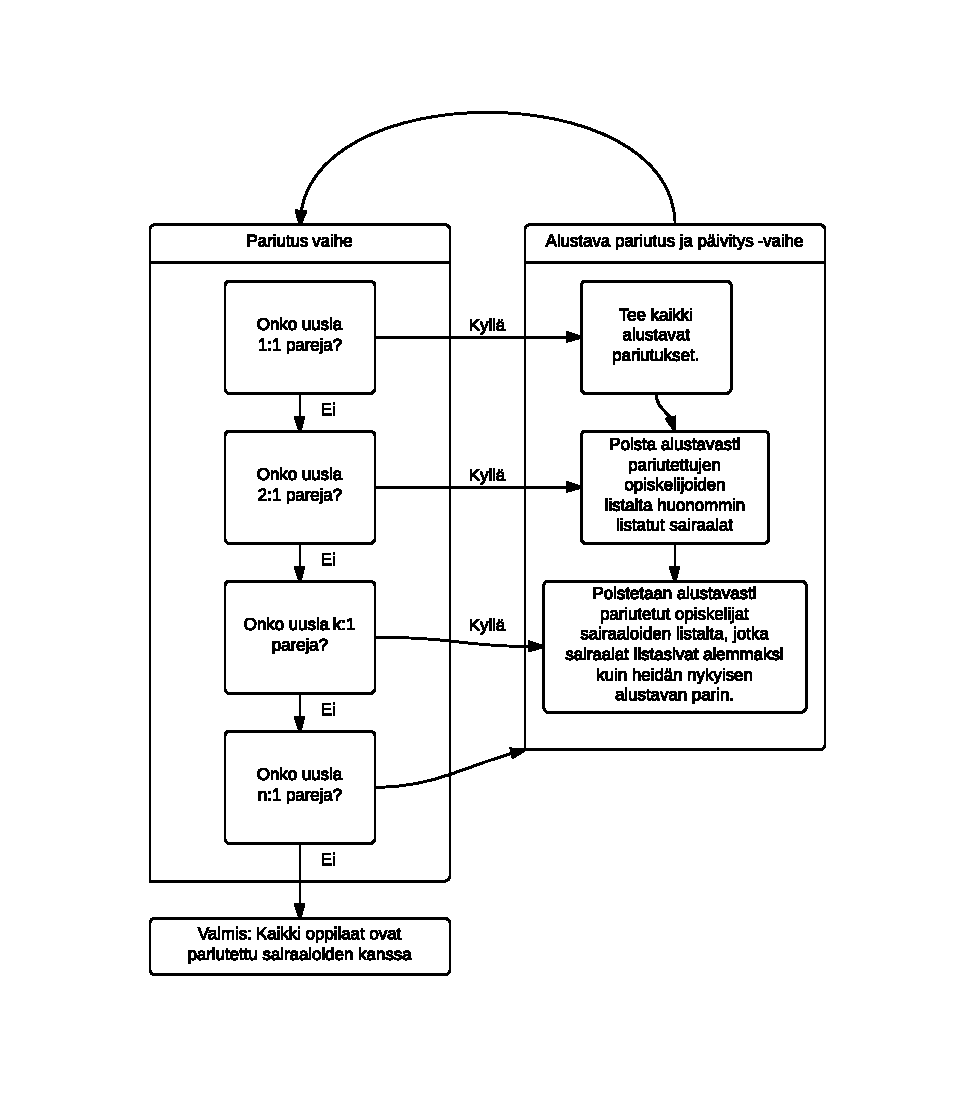
\includegraphics[scale=0.9]{NIMP}
\end{figure}
Verrattuna Gale--Shapley-algoritmiin toimintaperiaate on hyvin erilainen, mutta molemmat tuottavat vakaita pariutuksia. Algoritmin \ref{nimp} pariutuksien vakauden todistus löytyy lähteestä ja se sivuutetaan tässä.

\section{Strategiat avioliittopeleissä}
Avioliitto peliin osallistuvan henkilön todelliset mieltymykset voivat hyvinkin erota hänen ilmoittamistaan mieltymyksistä. Mieltymykset mitkä henkilö julkisesti ilmoittaa kutsutaan strategiaksi \cite[p, 592]{Balinski}, joka muiden henkilöiden strategioiden kanssa koostavat vakaan pariutuksen kyseisessä avioliittopelissä.

Esimerkiksi olkoon meillä nainen $n_1$, jonka aidot mieltymykset ovat seuraavat $m_1 > m_2 > m_3 > m_4$, pelistä ja miesten mieltymyksistä riippuen naisen on mahdollista päättyä kaikkien miesten kanssa avioliittoon. Jos nainen ilmoittaa mieltymyksikseen $m_1 > m_2$, ja ei edes harkitse avioliittoa miesten $m_3$ ja $m_4$ kanssa paranee naisen tilanne selvästi, ja avioliittopelissä hänen on mahdollista päätyä avioliittoon vain miehen $m_1$ tai $m_2$ kanssa.

Seuraavaksi näytetään, että rehellisyys on pätevä strategia, mutta mieltymysten muuntamisella voidaan saada henkilölle parempia pareja.

\begin{lem}\cite[p, 587]{Balinski}\label{bal-1}
	Olkoon olemassa pariutus $\mu$ ja $\mu^{'}$. Miehet $m \in M^{'} \subset M$ suosivat pariutusta $\mu$ verrattuna pariutukseen $\mu^{'}$, mutta miehet $m \notin M^{'}$ eivät, nyt on olemassa joku kaksikko $m$ ja $n$, missä $m \notin M^{'}$, joka estää pariutuksen $\mu$.
\end{lem}

$\Gamma$ edustaa todellista mieltymyslistaa, joukko $M^{'}$ miehiä, jotka väärentelevät mieltymyksiään ja $\Gamma^{'}$ mieltymyslistaa, joka ottaa nämä väärennetyt mieltymykset huomioon.

\begin{lem}\cite[p, 56]{gusfield1989stable}\label{strategy-gus}
	Ei ole olemassa vakaata pariutuksia suhteessa mieltymyksiin $\Gamma^{'}$, missä jokainen mies joukosta $M^{'}$ saa parin jota suosii ehdottomasti enemmän kuin pariaan pariutuksessa $M_0$.
\end{lem}

Todistukset löytyvät lähteistä ja sivuutetaan tässä.

\begin{lau}\cite[p, 593]{Balinski}
	Oletetaan, että $\Gamma$ edustaa jokaisen henkilön aitoa mieltymystä ja $\Gamma^{'}$ samoin, paitsi miesten $M^{'}$ osajoukon, joilla on vaihtoehtoinen mieltymys $\Gamma^{'}$:ssa. Ei ole olemassa vakaata pariutusta $\mu^{'}$ $\Gamma^{'}$:ssa jota kaikki miehet pitäisivät parempana kuin pariutusta $\mu$.
\end{lau}
\begin{proof}
	Oletetaan, että pariutus $\mu$ on miellyttävämpi kuin pariutus $\mu^{'}$ miehille $m \in M^{'} \subset M$. Lemman \ref{bal-1} mukaan täytyy olla olemassa pari $m$ ja $n$ missä $m \notin M^{'}$, joka estää pariutuksen $\mu$ mieltymyksillä $\Gamma$. Mutta miehen $m$ ja naisen $n$ strategiat ovat identtiset joukoissa $\Gamma$ ja $\Gamma^{'}$, joten $m$ ja $n$ on estepari myös mieltymyksellä $\Gamma^{'}$.
\end{proof}

Olkoon $M_0$ mies-optimaalinen pariutus suhteessa todellisiin mieltymyksiin $\Gamma$. Monessa avioliittopelissä tuloksia voidaan muunnella strategioilla vain silloin kun jokin osajoukko henkilöistä vääristelee yhdessä mieltymyksiä, eli he muodostavat \emph{koalition} ja tuottavat itselleen ja koalitiolle parempia pariutuksia.

\begin{lau}\cite[p, 58]{gusfield1989stable}
	Vaikka nais-orientoitunutta Gale--Shapley-algoritmiä (naiset kosii, miehet päättää) käytetään, voivat miehet pakottaa algoritmin tuottamaan mies-optimaalisia tuloksia antamalla väärennettyjä mieltymyksiä.
\end{lau}

\begin{proof}
	Jokainen mies $m$ väärentää mieltymyslistansa. Nämä miehet ilmoittavat, että huonompi nainen kuin $p_{M_0}(m)$ on hylättävä ja ei sovi miehelle pariksi, tämä tuottaa mieltymslistan $\Gamma^{'}$. Jos mies-orientoitunutta Gale--Shapley-algoritmiä käytetään mieltymyksille $\Gamma^{'}$ se tuottaa $M_0$, mies-optimaalisen pariutuksen mieltymyksille $\Gamma$. Edelleen, koska pariutuksessa $M_0$ jokaisella miehellä on huonoin mahdollinen pari suhteessa mieltymyslistaan $\Gamma^{'}$, on se ainoa mahdollinen vakaa pariutus tässä kontekstissa. Näinollen $M_0$ on vakaa pariutus jonka nais-orientoitunut Gale--Shapley-algoritmi tuottaa suhtessa mieltymyksiin $\Gamma^{'}$.
\end{proof}

Ylläolevalla strategialla on eräs vakaus ominaisuus joka rohkaisee miehiä toteuttamaan sovittu strategia. Oletetaan, että miehet sopivat keskenään ylläolevan kaltaisesta strategiasta, mutta ennen kuin väärennetty mieltymyslista julkaistaan jokin osajoukko koalitiosta päättää pettää koalition. Nämä miehet olettavat, että loput koalition miehet toteuttavat alkuperäisen strategian ja naiset antavat todelliset mieltymyksensä. Ongelmana pettäjillä on löytää optimoitu mieltymyslista, joka tuottaa heille vielä parempia pareja. Vaikka tälläistä petosta ei tapahdu jokainen mies voi olla huolissaan, että tälläinen petos tapahtuu hänen selkänsä takana ja epäröi osallistumistaan alkuperäiseen strategiaan, jossa kaikki miehet antoivat väärennetyt mieltymyslistat. Seuraava lause kertoo, että koalition on turha etsiä parempaa strategiaa ja näinollen miesten ei tarvitse huolehtia petoksista koalitioissa \cite{gusfield1989stable}.

\begin{lau}\cite[p, 58]{gusfield1989stable}
	Olkoon $M^{'}$ miesten osajoukko ja olkoon $\mu$ mikä tahansa pariutus missä jokainen mies joukosta $M^{'}$ suosii $\mu$-pariaan enemmän kuin $M_0$-pariaan. Olettaen, että jokainen mies joka ei ole joukossa $M^{'}$ ilmoittaa hänen $\Gamma^{'}$ listansa, ja jokainen nainen ilmoittaa heidän $\Gamma$ listansa, ei ole olemassa sellaista listojen joukkoja minkä $M^{'}$ voi ilmoittaa niin että $\mu$ olisi vakaa suhteessa ilmoitettuihin listoihin.
\end{lau}

\begin{proof}
	Oletetaan, että jokin osajoukko joukosta $M^{'}$ väärentää heidän sovitut mieltymyslistat luomalla mieltymykset $\Gamma_{M^{'}}$ aikaisemman ja sovitun $\Gamma^{'}$ mieltymyslistan sijaan. Nyt $M_0$ on ainoa vakaa pariutus mieltymyksille $\Gamma^{'}$, joten se on siis mies-optimaalinen pariutus molemmissa $\Gamma$:ssa ja $\Gamma^{'}$:ssa. Näinollen jos miehet joukossa $M^{'}$ parantelevat parejaan, suhteessa mieltymyksiin $\Gamma$, petoksen johdosta on kaikkien heidän saatava paremmat parit verrattuna mies-optimaaliseen pariutukseen mieltymyksillä $\Gamma^{'}$. Mutta Lemmassa \ref{strategy-gus} sanotaan, että miesten joukossa $M^{'}$ on mahdotonta ehdottomasti parantaa pariaan mieltymyksilla $\Gamma^{'}$ valehtelemalla.
\end{proof}

Täytyy huomauttaa, että ylläoleva strategia on hyväksyttävä vain avioliittopeleissä joissa hyväksytään parien kieltäminen.


% --- Back matter ---
%
% bibtex is used to generate the bibliography. The babplain style
% will generate numeric references (e.g. [1]) appropriate for theoretical
% computer science. If you need alphanumeric references (e.g [Tur90]), use
%
% \bibliographystyle{babalpha-lf}
%
% instead.

\bibliographystyle{babplain-lf}
\bibliography{ref}


\end{document}
